\documentclass[12pt]{article}
\usepackage{amsmath}
\usepackage{graphicx}
\usepackage{fancyhdr}
\usepackage{geometry}
\usepackage{float}
\geometry{a4paper}

% Set up header/footer
\pagestyle{fancy}
\fancyhead[L]{Test Data Science 1 - Classification}
\fancyhead[R]{Ángel Díaz Carral}

\title{Test Data Science 1 - Classification}
\author{Ángel Díaz Carral}
\date{\today}

\begin{document}

\maketitle

\begin{abstract}
This report describes the classification project based on an open dataset. The project aims to explore the use of machine learning models to classify images and compare the performance of standard Convolutional Neural Networks (CNN) with rotationally equivariant CNNs. The main hypothesis is that rotationally equivariant models can improve classification performance by avoiding the need for data augmentation and handling rotated images directly. The findings show that this approach can significantly enhance accuracy, particularly for image datasets where rotation is a key invariant feature.
\end{abstract}

\section{Introduction}
In this project, we use the MNIST dataset, a widely recognized dataset for handwritten digit classification. The dataset consists of 28x28 grayscale images of handwritten digits from 0 to 9. To make the problem more challenging for standard models, the images are rotated randomly between -180 and 180 degrees. The goal is to train different classification models and evaluate their performance, particularly focusing on the advantages of using rotationally equivariant models, which can inherently handle rotations without additional data preprocessing like augmentation.

\section{Exploratory Data Analysis (EDA)}
The dataset is composed of 60,000 training images and 10,000 test images. In the preprocessing stage, we rotated the images randomly between -180 and 180 degrees. Additionally, blurry images were filtered out to ensure the quality of the data used for model training. We then selected a random subset of 5\% of the original dataset to test the performance of our models, since even with this smaller set, we were able to achieve high classification accuracy.

\subsection{Visualizations}
Visual inspection of some rotated images reveals the complexity added by random rotations, which emphasizes the need for models that can handle rotational invariance. 

\begin{figure}[h!]
    \centering
    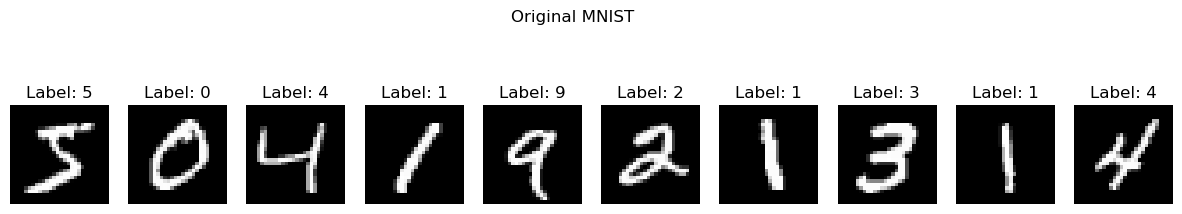
\includegraphics[width=1.0\textwidth]{pics/1output.png}
    \caption{Visualization of feature distributions}
\end{figure}

\begin{figure}[h!]
    \centering
    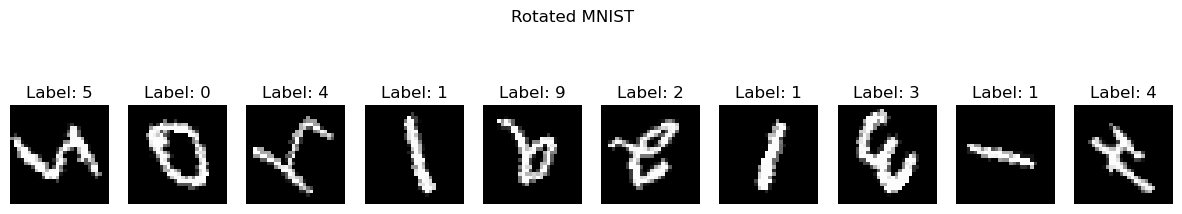
\includegraphics[width=1.0\textwidth]{pics/2output.png}
    \caption{Visualization of feature distributions}
\end{figure}

t-SNE is used to reduce the feature space to 2D, helping to visualize how the model clusters data points. The plot shows whether the model has learned meaningful feature representations and if different classes are well-separated or overlapping.

\begin{figure}[H]
\centering
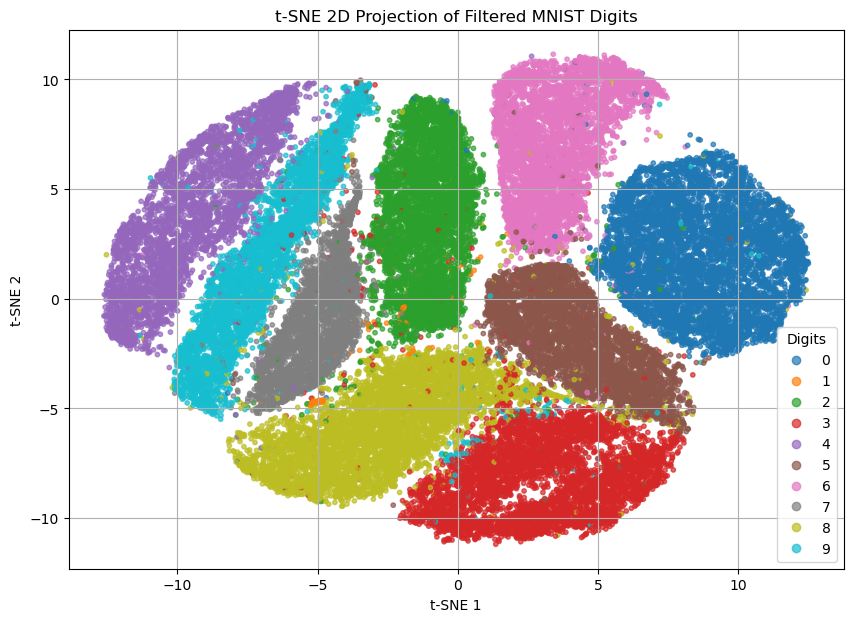
\includegraphics[width=0.6\textwidth]{pics/tsne.png}
\caption{t-SNE Visualization of Feature Space}
\end{figure}

\section{Model Selection and Training}
We experimented with the following models:

\begin{itemize}
    \item \textbf{Logistic Regression}: A simple linear model that, despite its simplicity, often serves as a baseline for comparison.
    \item \textbf{Convolutional Neural Networks (CNN)}: A standard deep learning model designed to handle image data, which learns spatial hierarchies of features.
    \item \textbf{Rotationally Equivariant CNN (RotCNN or E(2)CNN)}: A variant of CNN that is specifically designed to recognize patterns regardless of the rotation of the image. This model applies special convolutional layers that allow the network to preserve rotational symmetry and combines with the translational, already treated by CNNs. In \texttt{E(2)CNN}, rotation equivariance is achieved by modifying the convolution operation to act on rotated input feature maps using the Euclidean group \( E(2) \), which combines translations and rotations. Mathematically, this is expressed as:

\[
f_{\text{out}}(x) = \int_{E(2)} f_{\text{in}}(g^{-1} \cdot x) \cdot W(g) \, dg
\]

where \( g \in E(2) \) represents rotations and translations, ensuring the features transform consistently under rotation.
\end{itemize}

\subsection{Model Training}
The following steps were performed to train the model:

\begin{verbatim}
# Code to train the model
from sklearn.linear_model import LogisticRegression
from sklearn.model_selection import train_test_split

X = data.drop(columns='target')
y = data['target']

X_train, X_test, y_train, y_test = train_test_split(X, y, test_size=0.2, 
														random_state=42)

model = LogisticRegression()
model.fit(X_train, y_train)
\end{verbatim}

\section{Model Evaluation}
We evaluated the performance of the models using several metrics:

\begin{itemize}
    \item \textbf{Accuracy}: Measures the overall correctness of the model. It is the ratio of correct predictions to total predictions.
    \item \textbf{Precision}: Indicates the proportion of positive predictions that are actually correct. This metric is crucial in imbalanced datasets where false positives need to be minimized.
    \item \textbf{Recall}: Measures the proportion of actual positives that are correctly identified by the model. It is important when the cost of missing a positive instance is high.
    \item \textbf{F1-Score}: The harmonic mean of precision and recall. It is a balanced metric that provides a single value to evaluate model performance when precision and recall are both important.
\end{itemize}

We evaluate the models on the entire MNIST test set, which consists of 10,000 images. This is compared with the training set size, which was a subset of the original MNIST dataset, comprising only 5\% of the total 60,000 images. Despite using only 3,000 images for training, the models were able to achieve competitive performance on the full test set. This demonstrates the models' ability to generalize from a small training set, especially the RotCNN, which is more robust to rotations and spatial transformations.

The performance results on the test set were evaluated using accuracy, precision, recall, and F1-score metrics, as shown in the confusion matrices for each model. Despite the limited size of the training set, the models, particularly the RotCNN, show strong performance, confirming the effectiveness of rotationally equivariant architectures in handling rotated data.

\subsection{Results}

The results from the models are as follows:

\begin{itemize}
    \item Logistic Regression: Accuracy = 49\%, F1 Score = 0.48
    \item CNN: Accuracy = 82\%, F1 Score = 0.82
    \item RotCNN: Accuracy = 90\%, F1 Score = 0.88
\end{itemize}

Figures \ref{fig:log_reg}, \ref{fig:cnn}, and \ref{fig:rotcnn} show the confusion matrices for each model: Logistic Regression, CNN, and Rotational CNN (RotCNN). 

The results show that the RotCNN outperforms both CNN and Logistic Regression in terms of accuracy and F1 score. Its rotationally equivariant layer enables it to handle rotated images effectively. In contrast, Logistic Regression achieves only around 50\% accuracy, as it does not account for rotations. The CNN performs better than Logistic Regression, as it handle translational symmetries, but still lags behind the RotCNN.

\begin{figure}[H]
    \centering
    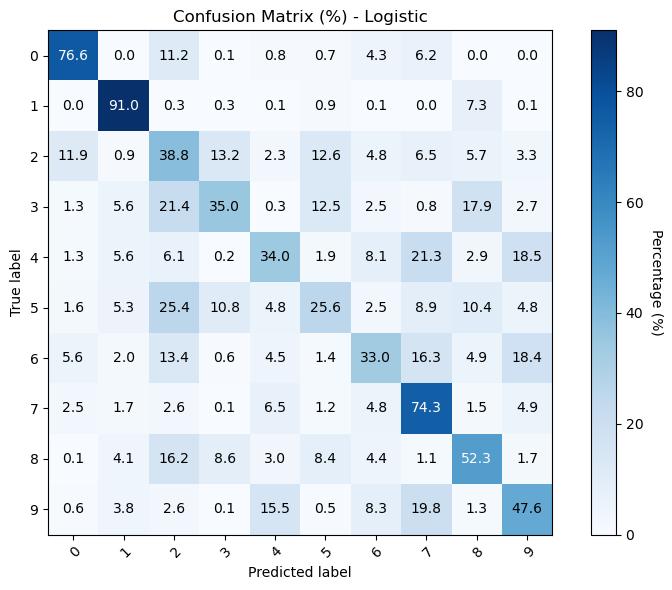
\includegraphics[width=1.0\textwidth]{pics/logtest.png}
    \caption{Confusion Matrix for Logistic Regression}
    \label{fig:log_reg}
\end{figure}

\begin{figure}[H]
    \centering
    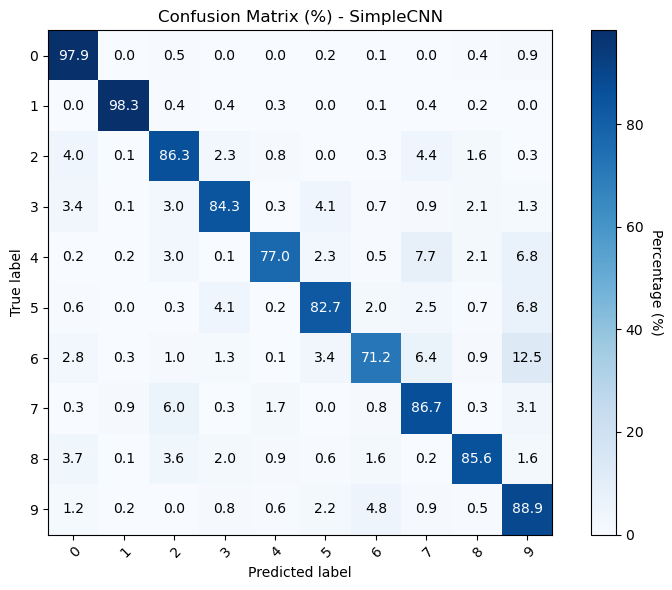
\includegraphics[width=1.0\textwidth]{pics/cnntest.png}
    \caption{Confusion Matrix for CNN}
    \label{fig:cnn}
\end{figure}

\begin{figure}[H]
    \centering
    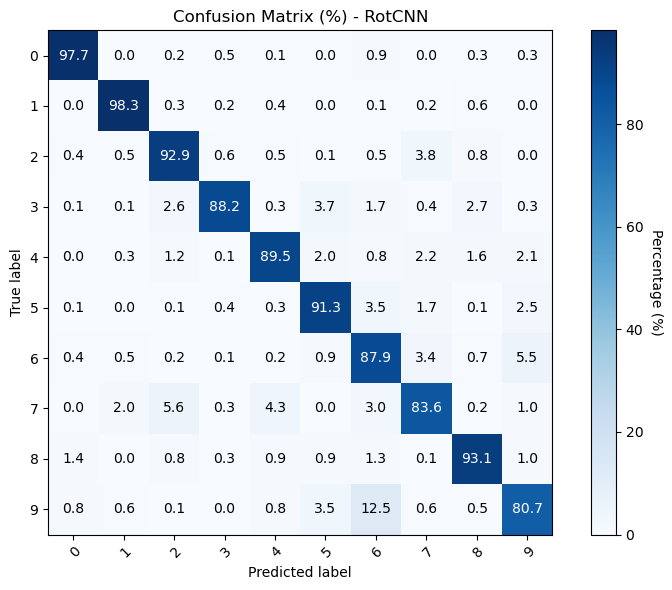
\includegraphics[width=1.0\textwidth]{pics/rotcnntest.png}
    \caption{Confusion Matrix for RotCNN}
    \label{fig:rotcnn}
\end{figure}

\section{Conclusions}
The rotationally equivariant CNN (RotCNN) significantly improves performance in this classification task. By directly handling rotated images without the need for explicit data augmentation, the RotCNN achieves higher accuracy and F1 score compared to traditional models. This is particularly advantageous when working with datasets where rotation is a key feature, as it allows the model to generalize better without the computational overhead of rotating the dataset manually. The results indicate that rotational equivariance is a valuable feature in image classification tasks involving rotations, and future work could further explore its application to more complex datasets and tasks.

\section{Deliverables}

The following files are provided in a python package to reproduce the analysis and deploy the trained model:

\begin{description}
    \item[\texttt{train\_model.py}] The script for training the model
    \item[\texttt{test\_model.py}] The script for evaluating the model
    \item[\texttt{model.pkl}] The trained model in pickle format
    \item[\texttt{structure.txt}] Directory structure of the project
\end{description}

Additionally, you can run the inference using the FastAPI-based API available at http://127.0.0.1:8000/prediction. 

For full access to the project, including code, data, and documentation, visit the repository on GitHub: 

\textbf{GitHub Repository:} The full source code, notebooks, Dockerfile, and documentation can be found at:
\begin{center}
\texttt{https://github.com/adiazcarral/ADC-TestDataScience-1}
\end{center}

\section{References}
\begin{enumerate}
    \item Dataset source
    \item Paper/Book for model selection
\end{enumerate}

\end{document}
